\documentclass[nobuilddate,nochap]{Docencia}

\title{Matemáticas II - Apuntes de clase}
\author{Departamento de Matemáticas}
\date{2019-2020}


\usepackage{tikz}
\usepackage{tikz-3dplot}
\usepackage{fancysprefs}
\usepackage{svg}


\usetikzlibrary{calc,patterns,angles,quotes}

\renewcommand{\ve}[1]{\ensuremath{\mathbf{#1}}}
\newcommand{\ud}[0]{\mathrm{d}}
\newcommand{\lgdlp}{Lugar geométrico de los puntos del espacio que equidistan de}


\tikzset{
    vector/.style = {
        thick,
        > = stealth',
    },
    axis/.style = {
        very thin,
        > = stealth',
    },
}


\begin{document}

\pagestyle{plain}

%%%%%%%%%%%%%%%%%%%%%%%%%%%%%%%%%%%%%%%%%%%%%%%%%%%%%%%%%%%%%%%%%%
%%%%%%%%%%%%%%%%%%%%%%%%%%%%%%%%%%%%%%%%%%%%%%%%%%%%%%%%%%%%%%%%%%
%%%%%%%%%%%%%%%%%%%%%%%%%%%%%%%%%%%%%%%%%%%%%%%%%%%%%%%%%%%%%%%%%%
%%%%%%%%%%%%%%%%%%%%%%%%%%%%%%%%%%%%%%%%%%%%%%%%%%%%%%%%%%%%%%%%%%
%%%%%%%%%%%%%%%%%%%%%%%%%%%%%%%%%%%%%%%%%%%%%%%%%%%%%%%%%%%%%%%%%%
%%%%%%%%%%%%%%%%%%%%%%%%%%%%%%%%%%%%%%%%%%%%%%%%%%%%%%%%%%%%%%%%%%
%%%%%%%%%%%%%%%%%%%%%%%%%%%%%%%%%%%%%%%%%%%%%%%%%%%%%%%%%%%%%%%%%%
%%%%%%%%%%%%%                                    %%%%%%%%%%%%%%%%%
%%%%%%%%%%%%%                                    %%%%%%%%%%%%%%%%%
%%%%%%%%%%%%%                                    %%%%%%%%%%%%%%%%%
%%%%%%%%%%%%%                                    %%%%%%%%%%%%%%%%%
%%%%%%%%%%%%%            DERIVABILIDAD           %%%%%%%%%%%%%%%%%
%%%%%%%%%%%%%                                    %%%%%%%%%%%%%%%%%
%%%%%%%%%%%%%                                    %%%%%%%%%%%%%%%%%
%%%%%%%%%%%%%                                    %%%%%%%%%%%%%%%%%
%%%%%%%%%%%%%                                    %%%%%%%%%%%%%%%%%
%%%%%%%%%%%%%%%%%%%%%%%%%%%%%%%%%%%%%%%%%%%%%%%%%%%%%%%%%%%%%%%%%%
%%%%%%%%%%%%%%%%%%%%%%%%%%%%%%%%%%%%%%%%%%%%%%%%%%%%%%%%%%%%%%%%%%
%%%%%%%%%%%%%%%%%%%%%%%%%%%%%%%%%%%%%%%%%%%%%%%%%%%%%%%%%%%%%%%%%%
%%%%%%%%%%%%%%%%%%%%%%%%%%%%%%%%%%%%%%%%%%%%%%%%%%%%%%%%%%%%%%%%%%
%%%%%%%%%%%%%%%%%%%%%%%%%%%%%%%%%%%%%%%%%%%%%%%%%%%%%%%%%%%%%%%%%%
%%%%%%%%%%%%%%%%%%%%%%%%%%%%%%%%%%%%%%%%%%%%%%%%%%%%%%%%%%%%%%%%%%
%%%%%%%%%%%%%%%%%%%%%%%%%%%%%%%%%%%%%%%%%%%%%%%%%%%%%%%%%%%%%%%%%%

\newpage\section{Derivadas y derivabilidad}

\subsection{Introducción y repaso}
\begin{defn}[Pendiente de una recta]
Sea la recta $y=mx+n$.

Se define \textbf{pendiente de la recta}, $m=\frac{\Delta y}{\Delta x}$
\end{defn}

\begin{defn}[Derivada\IS en un punto]
Se define $f'(a)$ como la derivada de $f(x)$ en el punto $x=a$.

\[f'(a) = \lim_{x\to a}\frac{f(x)-f(a)}{x-a} \overset{(1)}{=} \lim_{h\to 0}\frac{f(a+h)-f(a)}{h}\]

$(1): h=x-a \dimplies x=a+h$

\textit{Ver \fref{fig::funinterpretacionderivadapunto}}.
\end{defn}



\subsubsection{Interpretación geométrica de la derivada}

Ver \fref{fig::funinterpretacionderivadapunto}.

\begin{figure}[hbp]
\centering
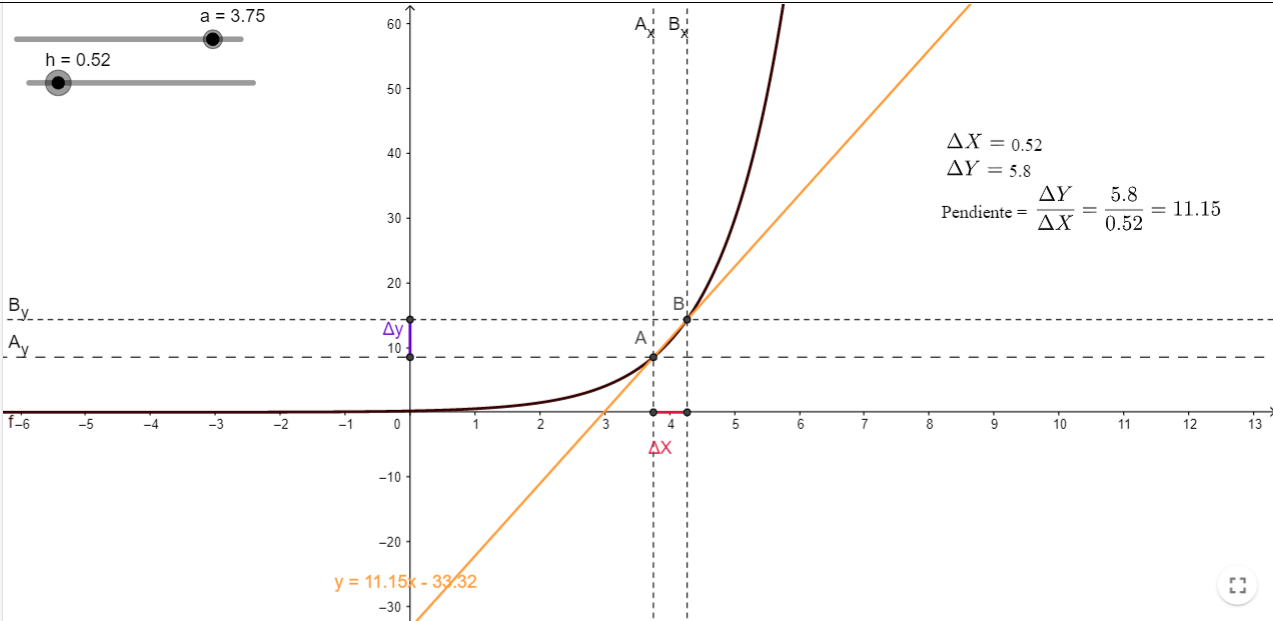
\includegraphics[scale=0.5]{img/DerivadaInterGeometrica}
\label{fig::funinterpretacionderivadapunto}
\caption{Interpretación geométrica de la derivada} Cuando $h\to0$, el punto $B$ se acercará cada vez más al punto $A$, dando lugar a la recta tangente. 
%
Para una mejor comprensión consultar la versión de Geogebra: https://www.geogebra.org/m/jwtw6mdt\#material/f52nQ7T5

\end{figure} 



\subsubsection{Derivabilidad}
\begin{defn}[Derivabilidad\IS en un punto]
\[f(x) \text{ derivable en } x=a\dimplies \exists f'(a)\]
\end{defn}


\begin{example}
Dada $f(x) = |x|$, calcula $f'(0)$.

\[
f(x) = \begin{cases}x&\text{ si } x>0 \\ -x & \text{ si }x\leq 0\end{cases}
\]

Calculamos:

\[
\lim_{x\to 0}\frac{f(x)-f(0)}{x-0} = \begin{cases}
\displaystyle\lim_{x\to 0^+} \frac{f(x)}{x} = \displaystyle\lim_{x\to 0^+} \frac{x}{x} = 1\\\\
\displaystyle\lim_{x\to 0^-} \frac{f(x)}{x} = \displaystyle\lim_{x\to 0^-} \frac{-x}{x} = -1
\end{cases}
\]

\label{derivEjemplo}

Los límites laterales no coinciden, por lo tanto, $\nexists \displaystyle\lim_{x\to 0}\frac{f(x)-f(a)}{x-a} \dimplies \nexists f'(a)$
\end{example}


\begin{prop}
$f(x)$ derivable en $x=a \implies f(x)$ continua en $x=a$
\obs El recíproco no es cierto. Basta comprobar el ejemplo \ref{derivEjemplo} ($f(x) = |x|$ es continua en $x=0$, pero no derivable en $x=0$).
\end{prop}

\begin{defn}[Derivabilidad\IS en un intervalo abierto]
\[f(x) \text{ derivable en } (a,b) \dimplies \forall c\in(a,b) \exists f'(c) \]
\end{defn}

\begin{defn}[Dominio de derivabilidad]
El dominio de derivabilidad de una función $f(x)$ es el mayor conjunto en el que la función es derivable.
\end{defn}

\obs $Dv(f) \neq D(f')$. Baste pensar en $f(x) = ln(x)$ cuya $f'(x) = 1/x$. En esta función, $D(f) = (0,\infty); Dv(f) = (0,\infty)$ pero $\{x\in \real / \exists \rfrac{1}{x}\} = \real - \{0\}$

\begin{example}
$f(x) = |x|$ no es derivable en $x=0$.

El dominio de derivabilidad de $f(x)$ es $\real-\{0\}$
\end{example}


\paragraph{Derivabilidad lateral:} De la misma manera que existía la \textit{continuidad lateral}, también podemos hablar de \textit{derivabilidad lateral}. 

\begin{defn}[Derivada lateral]
La derivada lateral de $f$ en $x=a$ por la derecha, escrita $f'(a^+)$, si existe:

\[f'(a^+) = \lim_{h\to 0^+} \frac{f(x+h)-f(x)}{h}\]

La derivada lateral de $f$ en $x=a$ por la izquierda, escrita $f'(a^-)$, si existe:

\[f'(a^-) = \lim_{h\to 0^-} \frac{f(x+h)-f(x)}{h} =  \lim_{h\to 0^+} \frac{f(x-h)-f(x)}{-h}\]

\obs Esta última igualdad se debe a que $h\to 0^-\implies h<0$. Si resulta menos confuso, puede elegirse trabajar siempre con $h>0$ y así los signos quedan explicitados.
\end{defn}

\obs Interpretación geométrica.

\begin{problem} Estudia la derivabilidad en $x=0$ de la función 
\label{prb::derivab1}
\[f(x) = \begin{cases} x^2+3x & \text{ si } x\leq 0\\ 3·\left(\frac{x^2+x}{x+1}\right)&\text{ si } x>0\end{cases}\]
\solution

$f(x)$ será derivable en $x=0$ si $\exists f'(0)$. Dado que $f(x)$ está definida a trozos, calculamos la derivadas laterales.

\[f'(0^-) = \lim_{h\to 0^+} \frac{f(0-h)-f(0)}{-h} = \lim_{h\to 0^-} \frac{(0-h)^2+3·(0-h)-(0^2+3·0)}{-h} = \lim_{h\to 0^-} \frac{h(h-3)}{-h} = +3\]
\[f'(0^+) = \lim_{h\to 0^+} \frac{f(0+h)-f(0)}{h} = \lim_{h\to 0^+} \frac{3·\frac{(0+h)^2+(0+h)}{0+h+1} - (0^2-3·0)}{h} = \lim_{h\to 0^+} \frac{3·\frac{h^2+h}{h+1}}{h} = \]
\[=\lim_{h\to 0^+} \frac{3·h·(h+1)}{h(h+1)} = 3 \]

\textbf{Conclusión:} Dado que  $f'(0^-) \eq f'(0^+) \implies f'(0) = 3$, por lo que la función es derivable en $x=0$.

% \begin{figure}[h!]
% \centering
% 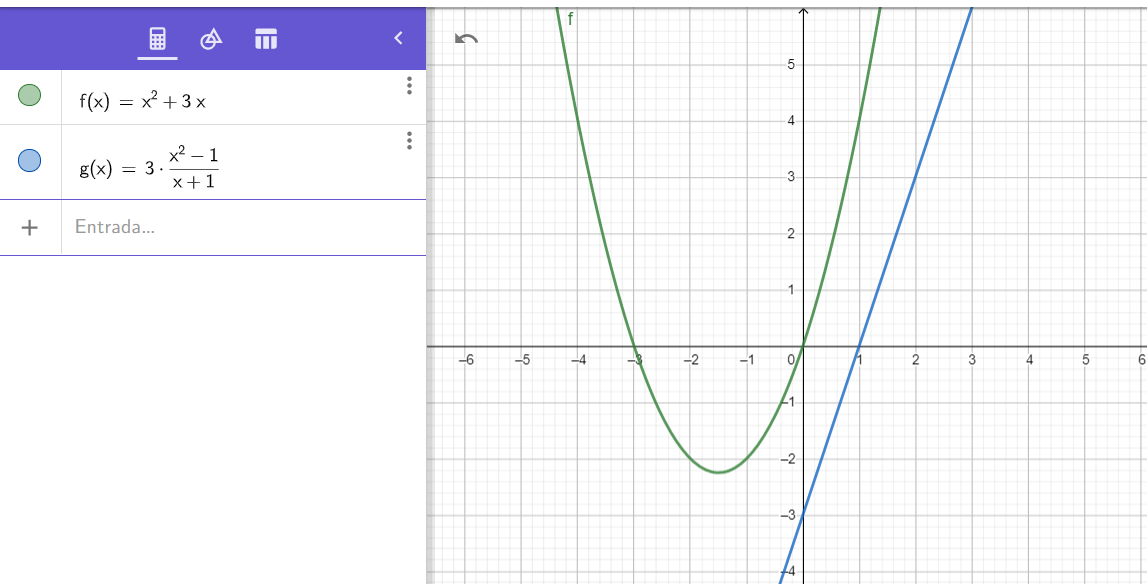
\includegraphics[scale=0.5]{img/DerivabilidadEjer1}
% \label{fig::DerivabEjer1}
% \caption{Representación gráfica del problema \ref{prb::derivab1}.}
% Claramente la derivada en $x=0$ no puede existir, dado que la función no es continua.
% \end{figure}

\obs También podríamos haber calculado la derivada lateral por la izquierda de la siguiente manera:

\[f'(0^-) = \lim_{h\to 0^-} \frac{f(0+h)-f(0)}{h} = \lim_{h\to 0^-} \frac{h^2+3·h-(0^2+3·0)}{h} = \lim_{h\to 0^-} \frac{h(h+3)}{h} = +3\]

\obs También podríamos haber calculado la derivada lateral por la izquierda de la siguiente manera:

\[f'(0^-) = \lim_{x\to 0^-} \frac{f(x)-f(0)}{x-0} = ... = +3\]


\end{problem}

\begin{prop}
$f(x)$ derivable en $x=a \implies f(x)$ continua en $x=a$
\end{prop}


\begin{prop}
\[
\left.\begin{array}{c}
f(x) \text{ continua en } x=a\\
f'(a^+) = f'(a^-)\end{array}\right\}\implies \exists f'(a) = f'(a^+) = f'(a^-)
\]
\end{prop}


\begin{problem} Estudia la derivabilidad en $x=0$ de la función 

\[f(x) = \begin{cases} x^2+3x & \text{ si } x\leq 0\\ \rfrac{3}{2}x^2+3x&\text{ si } x>0\end{cases}\]
\solution



Podemos calcular la función por ramas ya que, en cada rama, es una función derivable en su dominio por ser polinómica y racional respectivamente, a excepción del $x=0$. Ese valor, tendremos que estudiarlo a parte.

\[f'(x) = \begin{cases} 2x+3 & \text{ si } x< 0\\ 3x+3 &\text{ si } x>0\end{cases}\]

Ahora estudiamos 

$$f'(0^+) = \lim_{x\to 0^+} f'(x) = \lim_{x\to 0^+} 3x+3 = 3$$


$$f'(0^-) = \lim_{x\to 0^-} f'(x) = \lim_{x\to 0^-} 2x+3 = 3$$


¿Podemos asegurar que como $f'(0^+) \neq f'(0^-)$, la función no es derivable en $x=0$?

Esto solo será verdad \textbf{si f(x) es continua en $x=0$}.

Comprobamos que $f(x)$ es continua en $x=0$ porque...

\end{problem}



% \begin{problem}[Página 43, 14.]
% ¿Es la siguiente función derivable en $x=-2,x=0,x=2$?

% \[f(x) = \begin{cases}
% x^2 & \text{ si } x<-2\\
% -4(x+1) & \text{ si } -2<x\leq0\\
% 3x^2-4 & \text{ si } 0<x\leq2\\
% 12x+1 & \text{ si } x>2
% \end{cases}\]
% \solution
% \end{problem}

% \begin{problem}[Página 56, ejercicio 78.]
% Dada la función $f(x)$, calcula $a,b,c\in\real$ para que la función sea derivable en $x=1$, sabiendo que $f(0) = f(4)$.
% \solution

% Solución: $a=-\rfrac{7}{4}; b=1; c=\rfrac{1}{4}$

% \begin{figure}[h!]
% \centering
% 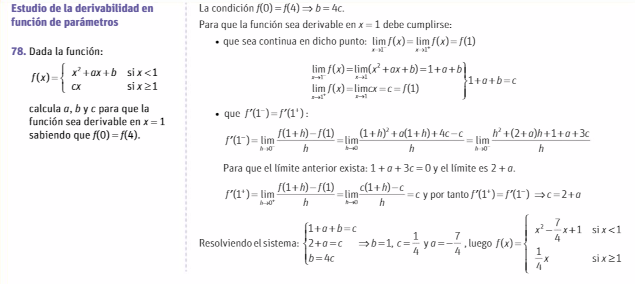
\includegraphics[scale=1.1]{img/DerivabilidadEjer5678}
% \label{ejercicioDerivabilidad}
% \caption{Ejercicio sacado del libro de SM}
% \end{figure}

% \end{problem}



\subsubsection{Función derivada}

\begin{defn}[Función derivada]
Dada $\appl{f}{D(f)\subset\real}{\real}$. Sea $Dv(f)$ el dominio de derivabilidad de $f$.

La función derivada denotada por $\appl{f'(x)}{Dv(f)\subset\real}{\real}$ hace corresponder a cada $a\in Dv(F)$ el valor $f'(a)$.
\end{defn}

% \begin{table}[hbp]
% \centering
% \begin{tabular}{|c|c|}\hline
% Función & Derivada\\
% \hline
% a&b\\\hline
% \end{tabular}
% \caption{Tabla de derivadas}
% \label{tbl::Derivadas}
% \end{table}

% \begin{problem}

% \begin{itemize}
% 	\item 51.58 (2 trigonométricas inversas)
% 	\item 59.113 (8 variadas. Solo la h tiene una trigonométrica inversa.)
% 	\item 57.79-81 (Ejercicios resueltos)
% \end{itemize}

% \solution
% \end{problem}


\subsection{Aplicaciones de la derivada}

\subsubsection{Recta tangente y recta normal}

\paragraph{Ecuación de la recta tangente:} Utilizando la ecuación de la recta punto-pendiente y la interpretación gráfica de la derivada (ver \ref{fig::funinterpretacionderivadapunto}), se obtiene fácilmente la siguiente ecuación:

\begin{mdframed}
	\begin{equation}
		\label{eq::rectatangente}
		\text{Recta tangente a }f(x)\text{ en }x_0 \to y-f(x_0) = f'(x_0)·(x-x_0)
	\end{equation}
\end{mdframed}

\begin{problem}
Demuestra que la recta $y=-x$ es tangente a la curva dada por la ecuación: $y=x^3+6x^2+8x$
\solution

Consideramos $f(x) = x^3-6x^2+8x \to f'(x) = 3x^2-12x+8$.

Buscamos $c\in\real\tq f'(c) = -1$.

\[
	3c^2+12c+8=-1 \dimplies \begin{cases}c_1 = 1\\c_2=3\end{cases}
\]

Los posibles puntos de tangencia son $P_1(c_1,f(c_1)) = (1,3)$ y $P_2(c_2,f(c_2)) = (3,-3)$.

Es necesario comprobar que dichos puntos son realmente de tangencia, es decir, que pertenecen a la recta y a la gráfica.

\[P_1: 3\neq -1 \implies \text{ no pertenece a la recta}\]
\[P_2: -3\eq -3 \implies \text{ sí pertenece a la recta}\]

\textbf{Conclusión: } El punto de tangencia de la recta $y=-x$ a la gráfica $f(x) = x^3-6x^2+8x$ es $P_2(3,-3)$
\end{problem}

\paragraph{Ecuación de la recta normal:} Dos rectas dadas, en 2 dimensiones, $r: y=m_rx+n_r\quad;\quad s:y=m_sx+n_s$ son perpendiculares si y sólo si $m_r·m_s = -1 \dimplies m_s = \rfrac{-1}{m_r}$.
%
Aplicando este resultado a la fórmula de la recta tangente anterior, tenemos:


\begin{mdframed}
	\begin{equation}
		\label{eq::rectatangente}
		\text{Recta normal a }f(x)\text{ en }x_0 \to y-f(x_0) = \rfrac{-1}{f'(x_0)}·(x-x_0)
	\end{equation}
\end{mdframed}




\end{document}
